\documentclass[a4paper, 12pt]{article}
% to add double-side margins
% \documentclass[a4paper, 12pt, twoside]{article}

\addtolength{\oddsidemargin}{-0.5in}
\addtolength{\evensidemargin}{-0.5in}
\addtolength{\textwidth}{1in}
\addtolength{\topmargin}{-0.5in}
\addtolength{\textheight}{1in}

\usepackage{amsmath}
\usepackage{algorithm}
\usepackage{algpseudocode}
\usepackage{fancyhdr}
\usepackage{float}
\usepackage{subfig}
\usepackage{enumitem}
\usepackage{appendix}

\usepackage{graphicx}
\graphicspath{ {images/} }

\usepackage{etoolbox}
\patchcmd{\thebibliography}{\section*{\refname}}{}{}{}
\setitemize{labelsep=0.5cm}
\setenumerate{labelsep=0.5cm}


\setlength{\parskip}{12pt}
%\title{Creating a Predictable Interconnection Network for General-Purpose Parallel Architectures}
\title{Reducing the Number of Collisions Between Communication Data Packets in General-Purpose Parallel Architectures}
\author{Benjamin Tovar Matthews}

\begin{document}

\setcounter{page}{0}
\maketitle

\begin{abstract}

\end{abstract}

\thispagestyle{empty}
\newpage
\pagenumbering{arabic}
\setcounter{tocdepth}{2}
\tableofcontents
\newpage
\listoffigures

\newpage
\section{Introduction}

\subsection{Definitions}

This thesis includes a number of terms that have been clarified below to avoid any potential ambiguity.
\begin{itemize}[leftmargin=0cm]

\item[] \textbf{Processor}: An integrated circuit which contains at least an arithmetic logic unit (ALU), registers, and a block of memory. Used to execute instructions outlined by programming code.

\item[] \textbf{Network}: A number of processors connected together by physical wires and intermediate nodes, allowing each processor to communicate with others in the network.

\item[] \textbf{Link}: A single wire in the network connecting either two processors, a processor and an intermediate node, or two intermediate nodes.

\item[] \textbf{Routing algorithm}: The algorithm that decides which links in the network are to be used when a communication is required between two processors on the network.

\item[] \textbf{Collision}: When two packets of communication data in the network try to use the same link at the same time, resulting in one of the packets having to wait until the link becomes free again before continuing its transmission.

\end{itemize}

\subsection{Outline of the problem}
\label{sec:problem_outline}

The world of computer programming is currently undergoing a paradigm shift from sequential programming to parallel programming. Sequential programs execute their set of instructions one after another in order, which means they can be run using a single processor. Parallel programs on the other hand include sections of instructions that can be executed independently from one another, which means they can be run on more than one processor in parallel. Applying parallelism to a sequential program means that the execution time of the program is reduced -- providing the program has independent sections suitable for parallel execution -- because some of the computation is being carried out concurrently.

However parallel computing is not without its drawbacks. While parallel programs are generally faster than sequential programs, they require more hardware and suffer larger overhead costs in order for the program to be executed correctly. In other words, a fully parallel version of a sequential program executed on $n$ processors will not run $n$ times faster than the sequential program runs on one processor, because of the additional overheads that parallelism introduces.

The main source of overhead during execution of a parallel program is communication between processors. Communication is an essential part of parallel computing because it allows processors to share their calculated data with the other processors they are working in collaboration with, which is necessary in almost all parallel programs. This communication is facilitated by a network of links which carry communication data from processor to processor. It is in these physical links where the majority of the overhead associated with parallel computing is sourced, resulting in slower execution time and reduced efficiency of parallel programs.

Ideally, a fully parallelised version of a sequential program would result in a linear speedup based on the number of parallel processors involved in the computation. However, due to the added overheads of parallelism, this is currently not the case. This thesis focuses on trying to reduce the significance of this overhead so that linear speedup due to added parallelism is more realistically achievable.

\subsection{Possible optimisations to current solutions}
\label{sec:possible_optimisations}

One optimisation that has become a lot more accessible in the last few years is the replacement of traditional copper wires in the network with optic cables, making the network photonic. This means that instead of data being transmitted over the network in the form of differing voltages of electric current, it is transmitted as pulses of light, which makes the network latency a function of the speed of light (approximately $3.0 \times 10^8 $ m/s), and eliminates inefficiencies such as friction between the electric current and the copper wire. However, while network latency of the speed of light sounds sufficient, in some cases it can still act as the computational bottleneck. An average modern CPU is manufactured with a clock speed of around 2.0 GHz, which equates to $2.0 \times 10^9$ clock cycles per second. This means that in 0.5 nanoseconds -- the time taken for one clock cycle to be carried out on this CPU -- light only travels around 15cm. This may be sufficient to carry out communication in one clock cycle in smaller networks, but for larger networks such as supercomputers which may have links spanning several metres, communication can take a lot longer. However, current research suggests that no advancement of the speed of light is possible at present, meaning that, for the time being at least, optimisations in the network must be sourced from elsewhere. 

Another possible optimisation involves increasing the efficiency of the way in which data is transmitted across the network. When lots of communication is being carried out concurrently by multiple processors, links in the network will inevitably begin to fill up leading to a situation where more than one piece of data tries to use the same link at the same time to advance towards its destination. This is known as a collision in the network. Sending both pieces of data down the same link not physically possible, meaning that one of the pieces of data is forced to wait for the link to become vacant again before continuing towards its destination, resulting in increased network latency \cite{Lam04}. This suggests that the fewer collisions that happen in the network, the lower the average network latency and the more efficiently communication data can be transmitted, making reducing the number of collisions in the network a possible strategy for optimising the execution time of parallel programs.

A third possible optimisation of current networks involves changing the way data is stored for each processor in the network. There is some variation between models and manufacturers, but a typical modern processor has access to four blocks of memory known as the memory hierarchy: CPU registers, cache memory (SRAM), main memory (DRAM) and the hard disk \cite{Toy86}. The memory stores towards the top of the hierarchy allow the processor the quickest access to their data with limited storage capacity, whereas the memory stores towards the bottom of the hierarchy offer the largest stores of data but with slower access rates. This suggests that in terms of program efficiency, it is profitable to store as much data as high up the memory hierarchy as possible, meaning that the time taken by the processor to access data is reduced. It could also suggest that increasing the memory capacity of the stores towards the top of the hierarchy, the cache for example, might increase the efficiency of the processor. However, increasing the cache size would result in an increased number of memory addresses, which would subsequently mean that the processor would take longer to find and access a given address which reduces the effect of having cache memory in the first place. This means that a compromise between size and speed must be found, and further research into that area could result in more efficient processors and an increase in the efficiency of parallel programs which use these processors. 

\subsection{Motivation}

Moore's law states that processing power should approximately double every two years \cite{Moo65}. In terms of parallel processors, this performance increase can be acquired by either increasing the number of transistors in each processor, or by increasing the number of processors used for parallel computation. However both of these solutions are flawed; in recent years the performance of serial processors has plateaued (for reasons described in section \ref{sec:need_parallelism}), and while adding more processors to the network may increase the overall processing power, it also increases the overhead costs making the processing less efficient as well as bearing a significant financial cost. If a solution can be found that increases the efficiency of parallel computation without the need of large numbers of added processors, this could potentially save hardware manufacturers a lot of money while still allowing them to emulate the advancement of Moore's law.

\subsection{Purpose}

The main aims of the thesis are outlined below:
\begin{itemize}
	\item Devise a solution to the problem of efficiency in general-purpose parallel architectures documented in section \ref{sec:problem_outline}.
	\item Create an emulation of a network, including multiple processors which are able to carry out message passing instructions to each other. Parallelism in this network should be at least emulated.
	\item Deploy the solution on this emulated network. The improvement that the solution provides should be documented by the program as a quantitative, measurable output.
	\item Ensure that the network remains universal so that the solution can be applied to any network topology (explained in section \ref{sec:topologies}).
	\item Ensure that the network remains scalable so that the solution can be applied to a network with any number of parallel processors in collaboration.
\end{itemize}

\subsection{Outline of the following chapters}

The remainder of the thesis is structured as follows:
\begin{itemize}[leftmargin=0cm]
	\item[] \textbf{Chapter 2}: A background chapter to introduce to some of the fundamental concepts discussed in the thesis.
	\item[] \textbf{Chapter 3}: An outline of the proposed solution and a detailed specification of requirements for this solution.
	\item[] \textbf{Chapter 4}: The design of the network and the solution, and a description of how the solution will be deployed on the network to produce meaningful results.
	\item[] \textbf{Chapter 5}: The implementation of the network and the solution.
	\item[] \textbf{Chapter 6}: Testing of the network to ensure that it works correctly.
	\item[] \textbf{Chapter 7}: Experimentation to show whether the solution produces the desired increase in network efficiency.
	\item[] \textbf{Chapter 8}: A conclusion of the work done in the thesis and suggestions of further work that could be carried out in this field.
\end{itemize}

\newpage
\section{Background}

This chapter describes some of the fundamental concepts needed to understand what is trying to be achieved with this project. It starts off with an introduction to the concept of parallelism. It then goes on to study parallel architecture in more depth, particularly the role that the interconnection network has in the system. Finally, it looks at some examples of modern general-purpose parallel architectures, and how the interconnection network provides communication between processors.

\subsection{General-purpose processors: a need for parallelism}
\label{sec:need_parallelism}

In the beginning processors were designed and built in a serial manner, using a single core, a single block of memory and a single set of instructions executed one after another. This setup is referred to as a SISD (single instruction, single data) architecture, a term defined in Flynn's Taxonomy as one of four classifications of processor architecture \cite{Fly72}. This architecture suited early processors because it was easy to implement, and expectations of processing performance were not as demanding as they have become today because very few general-purpose machines existed. However, as more research was conducted and use of general-purpose machines became more common, it was clear that optimisation of this architecture was required to boost the performance of processors that were executing increasingly more complex programs and calculations. 

At first, work was able to be done using the SISD architecture to increase processing performance. Techniques such as the pipelining of the fetch-execute cycle were introduced, which allowed different parts of the cycle to be carried out on different instructions in a concurrent manner, resulting in an instruction being executed on every clock cycle \cite{Iba08}. This is an important increase compared to the whole fetch-execute cycle being carried out fully on each instruction before moving on to the next; assuming each step in the fetch-execute cycle takes one clock cycle, the resulting performance would be one instruction executed every three clock cycles. This suggests pipelining increased processor performance by a factor of three.

However, techniques such as pipelining were not the main source of increased performance for SISD architectures. It was clear that clock speed determined the speed at which instructions were executed, so the faster the clock speed, the better the resulting processor performance. To increase clock speed, the voltage of the power supply to the processor needed to be increased. This was not much of a problem, so the voltage was slowly increased to match performance increase stated by Moore's law, which observes that the number of transistors (therefore the processing power) in a processor should double every two years \cite{Moo65}. Figure \ref{fig:cpu_trends} below shows the rise of power input, clock speed and processor performance of Intel processors in the last 40 years or so.

\begin{figure}[H]
\centering
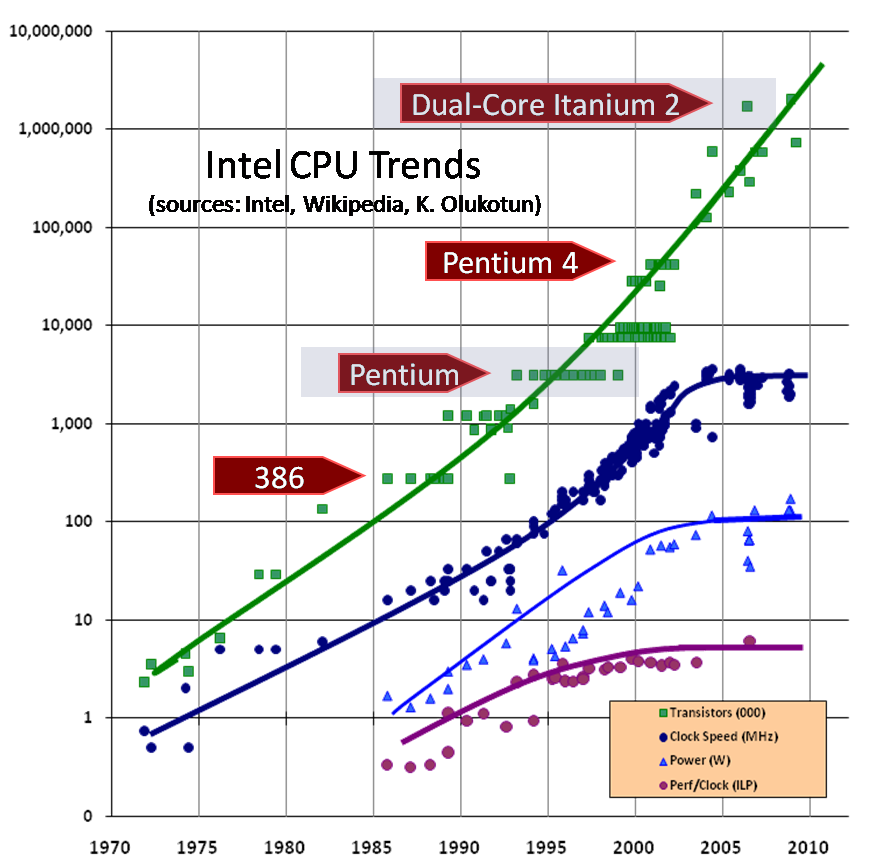
\includegraphics[width=\textwidth]{trend_graph.png}
\caption[A subset of Intel CPU introductions between 1970 and 2010]{A subset of Intel CPU introductions between 1970 and 2010. \cite{Sut05}}
\label{fig:cpu_trends}
\end{figure}

The number of transistors, shown by the green line, shows that processor performance is consistently growing at an exponential rate, which matches Moore's law. The growth of power input and clock speed are shown by the light and dark blue lines respectively. It can be seen that these values also rose exponentially, until about 2002 when they both seem to level out. This point indicates the beginning of the use of parallelism in general-purpose processors.

The problem with increasing the voltage input to the processor is that a by-product of power is heat. This was not a problem when the technique was originally applied, as cooling systems such as fans were sufficient to manage the heat output. However, as more and more power was required to increase clock speed further for each new build, the processor was giving off more and more heat until a level of heat was reached that could not be sufficiently cooled and became a danger to the computer and its environment \cite{Adv08}. This meant that processor performance matching Moore's law could not longer be attained by increasing clock speed; a new technique was required to continue growth of processing performance.

\subsection{An introduction to parallel systems}

This new technique was the use of parallelism within the processor. Operating on the principle that large problems can often be divided up into smaller, independent problems, parallel systems have more than one processing core that can each carry out an instruction on different pieces of data concurrently \cite{Got89}. With each instruction executed in parallel to another, the execution time of the instruction is 'hidden' meaning the overall runtime of the program is reduced compared to serial execution. This is the basis on which parallel systems achieve improved performance, without relying on an increase in clock speed.

Of course, this technique was not particularly new. It was used prior to 2002 for many years in the high-performance computing industry, where it was used in massively parallel supercomputers which executed large-scale calculations such as molecular dynamics and climate modelling. These machines were very specialist and not general-purpose, but their parallelism worked very well. This meant that when the time came, the technique could be taken and applied to general-purpose systems to give increased processing performance on machines that were available for use by the general public.

Most general-purpose parallel systems use a SIMD (single instruction, multiple data) architecture, another classification of processor defined in Flynn's Taxonomy \cite{Fly72}. This architecture works in a way that is best explained using a simple example of a calculation that it can perform. Imagine a $4 \times 4$ matrix of random integers, and a program that aims to find the product of these integers. A SISD architecture, which uses one core and one block of memory, would execute fifteen serial multiplications to find the product of the $4 \times 4$ matrix. However for a SIMD architecture with four cores, each with its own memory block, the $4 \times 4$ matrix can be split into four $4 \times 1$ matrices, one for each core in the processor. Parallel execution of three serial multiplications by each core can then be carried out, resulting in four partial product values which are then in turn multiplied by the master core to get the final value. Assuming each multiplication takes one clock cycle, the SISD architecture can complete the calculation in fifteen clock cycles, whereas the SIMD architecture can theoretically complete the calculation in six clock cycles. I say theoretically because parallel architectures are not as simple as serial architectures, and come with some overheads that have not yet been discussed. The main overhead associated with parallel architectures is communication between cores, which is the main focus of this paper.

\subsection{An introduction to interconnects}

Interconnects provide communication channels between cores working concurrently, and are an integral part of a parallel architecture. Let us look at the $4 \times 4$ matrix multiplication example again, this time in more detail.

The program starts off in the same way that a serial program would start, running on the master core only. Here, random integers are assigned to each position in the $4 \times 4$ matrix, arbitrarily in the case of this example. Once the matrix has been filled, the parallel section of the program can begin. The matrix is split up into rows, giving four $4 \times 1$ matrices. However for these matrices to be distributed between the four available cores, they need to be passed from the master core via an interconnect. The interconnect provides a path for data between cores, meaning the first $4 \times 1$ matrix can be passed from the master core to core[1], the second $4 \times 1$ matrix can be passed to core[2] and the third $4 \times 1$ matrix can be passed to core[3]. The fourth $4 \times 1$ matrix does not need to be passed to a different core, it remains on the master core (core[0]). Once all data has been distributed between cores, parallel processing begins as each core calculates the product of its section of the $4 \times 4$ matrix, resulting in four partial product values; one on each core. Again, interconnects are needed here to transport each partial product back to the master core, so that the final multiplication can take place. This is the end of the parallel section, and the final multiplication is done in serial resulting in the returned value of the program.

This is a very simplified example of the type of calculation parallel systems are used for, but it gives a good indication of how important interconnects are to the functionality of a SIMD architecture. However their use is not without its drawbacks, mainly the associated overheads that it adds to the system using it. For example in the program described above, extra computation is required by the system to specify a destination for each $4 \times 1$ matrix, to distribute the list of instructions to be executed by each core, and to specify the destination for each of the partial products. Another large overhead is the time taken to physically transport data across an interconnect wire. The speed of data transportation is restricted by the speed of light, roughly $3.0 \times 10^8$ m/s, and while this may seem more than sufficient for transportation rates of negligible time, let us consider the speed of modern processor clock speeds. An average clock speed in 2015 is around 2 GHz, which is equivalent to $2.0 \times 10^9$ clock cycles per second. So in one clock cycle, light travels roughly 15cm. This is not a very large distance, especially in larger scale supercomputers when interconnects may need to stretch tens or hundreds of metres. This suggests that, given the speed of modern processors, the majority of runtime in a parallel program is spent on data transfer rather than actual computation, which means that efforts to speed up the service that interconnects provide are essential for providing a further improvement of parallel processing performance.

\subsection{Interconnection networks}

An interconnection network is built up when a number of interconnects are used in a parallel architecture. In an ideal world, each core would be connected to every other core by a single interconnect, giving direct communication between all cores in a system. However in practice this is not feasible, as for every nth core added to the network, $n-1$ interconnects must also be added to maintain complete connection. This means that the number of interconnects scales by $n^2$ the number of cores, making this implementation non-scalable and not an option.

Instead, a sparsely-connected network must be used where each core is connected to a small number of other cores. As long as every core is reachable by every other core, which the network model requires, communication can then take place either directly between connected cores, or indirectly using more than one interconnect via intermediate cores. Switches can also be used in an interconnection network as intermediate nodes, which direct data down different paths in the network. These will be described in more detail later.

\subsection{Network topologies}
\label{sec:topologies}

A topology represents an abstracted layout of a network, in terms of cores/switches (nodes) and interconnects (edges). There are many different topologies that can be used, with even modern supercomputer manufacturers disagreeing about which one gives best performance \cite{Han14}. There are five main topologies: mesh, toroidal, hypercubic, tree and Clos.

\begin{figure}[H]
\centering
\subfloat[2D mesh] {
	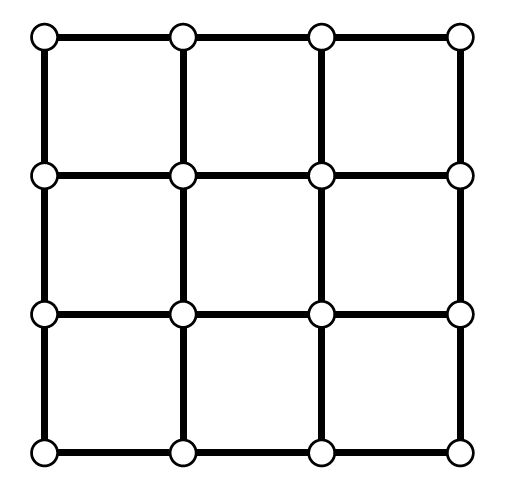
\includegraphics[width=65mm]{mesh_network.png}
}
\subfloat[2D torus] {
	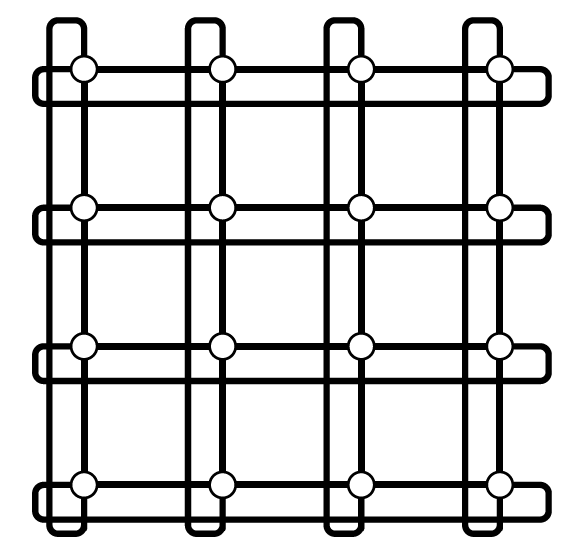
\includegraphics[width=65mm]{toroidal_network.png}
}
\newline
\subfloat[4D hypercube] {
	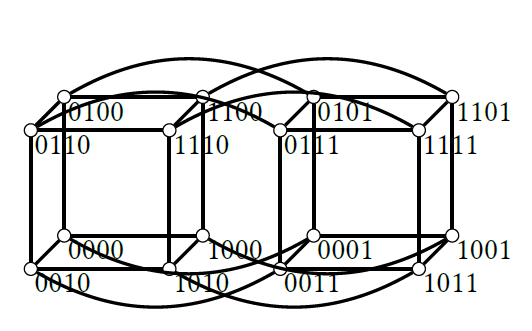
\includegraphics[width=65mm]{hypercubic_network.png}
}
\subfloat[Fat tree] {
	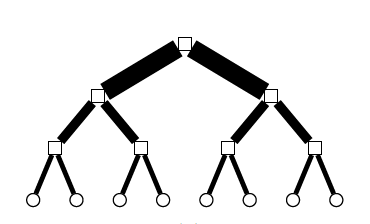
\includegraphics[width=65mm]{fat_tree_network.png}
}
\newline
\subfloat[Clos] {
	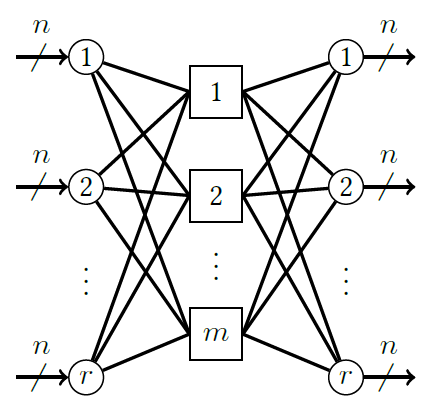
\includegraphics[width=65mm]{clos_network.png}
}
\subfloat[Bene\v{s}] {
	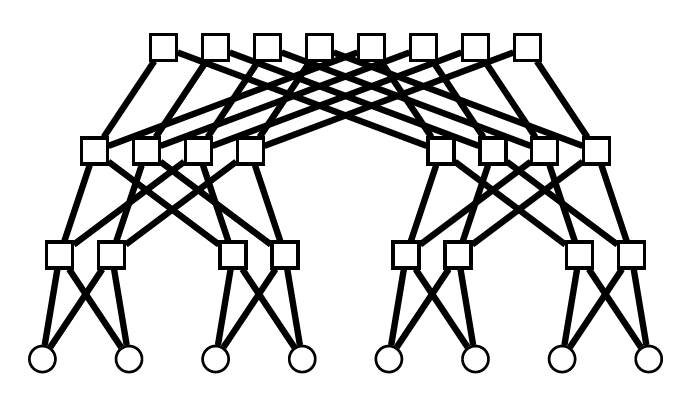
\includegraphics[width=65mm]{benes_network.png}
}
\caption[Different network topologies used in parallel architectures]{Different network topologies used in parallel architectures. \cite{Han14}}
\label{fig:topologies}
\end{figure}

Mesh and toroidal networks have a regular layout similar to arrays. Cores in mesh networks are only connected to adjacent positions in the array, with the cores in the middle of the array having more connections than the cores at the edge. Toroidal networks remove this non-uniformity, allowing cores at the edge of the array to 'wrap around' the array to connect to the adjacent node at the other end of the dimension.

Hypercubic networks have a symmetric and recursive structure. A $d+1$ dimensional hypercubic network can be constructed by connecting two d dimensional hypercubes by their matching cores. 

Tree networks have a root node connecting one or more child nodes, which in turn connect one or more child nodes until all nodes are connected. The fact that all nodes have the common root node means that every node is reachable, which is a requirement of a network topology. However because there is only one root node, traffic around this node can get quite busy when lots of communication is taking place. Fat trees address this problem, giving interconnects closer to the root of the tree more bandwidth so that more data can be transmitted on each clock cycle.

Clos networks were originally designed for use in telecommunications \cite{Clo53}. They use non-blocking switches to allow continuous transfer of data over multiple connections. Each connection has three stages: an ingress stage where data is sent from a core, a middle stage where data passes through one or more switching nodes, and an egress stage where data is received by the receiving core. The middle stage can be made up of further Clos networks, making a chain structure which gives more paths for each connecting nodes. Bene\v{s} networks are a type of Clos network, where each node is connected to exactly two other nodes \cite{Ben65}. Due to the symmetry of Clos and Bene\v{s} networks, they can be folded across the middle stage as shown in figure \ref{fig:topologies}f. This merges the ingress and egress stages by using bidirectional communications links, allowing more efficient traversal of the network.

\subsection{Routing}

A routing algorithm decides which path of a network the data is sent along during communication between two nodes. Ideally the shortest path between the two nodes is selected, however consideration of the state of the network should be taken into account to try and minimise link contention within the network. There are a number of different routing algorithms used in parallel systems, a selection of which are described below.

\subsubsection{Oblivious routing}

Oblivious routing ignores the state of the network when deciding which path should be chosen for communication. This means that it typically chooses the shortest path between two nodes, which can result in very poor use of the network in the worst case. However the worst case is an unusual scenario, and in the average case this algorithm can perform quite well with minimal overheads slowing down communication.

\subsubsection{Adaptive routing}

Adaptive routing aims to distribute communication paths across the network more evenly \cite{Dal03}. Each node uses the buffer occupancy in the nodes connected to it to choose the path with the least traffic, allowing data to be transmitted down the least congested path. However this technique is open to the risk of livelock, where the chosen path goes around in circles and the data does not progress towards its destination. This is obviously a problem, as data is not guaranteed to reach its destination in an acceptable time for efficient communication to take place.

\subsubsection{Two-phase randomised routing}

Two-phase randomised routing is another technique used to spread traffic uniformly over the network \cite{Val90}. It selects a random intermediate node somewhere in the network, and then ensures that data passes through this node on its way to its intended destination. As the name suggests, communication is split into two phases: sending the data to the intermediate node, and forwarding the data on to the destination node. Both of these phases use oblivious routing, meaning that data generally travels twice the average path length, but the addition of the random element tends to distribute traffic evenly over the network and improves communication efficiency.

\subsection{Switching}

A switching scheme handles the way in which network resources are used during communication. Switches are included in a network as intermediate nodes that forward data along a specified route to its destination node. There are a number of different switching schemes used in parallel systems, a selection of which are described below.

\subsubsection{Packet switching}

Packet switching is a very commonly used switching scheme. It splits the piece of data to be transmitted up into fixed length parts called packets, and then each of these packets is transmitted independently of one another to their destination. Once all the packets have reached their destination, the data is then reassembled and reconstructed ready for use by the node. The fact that packets are send independently means that in some situations they can be sent concurrently down different paths of the network, improving communication efficiency.

\subsubsection{Circuit switching}

Circuit switching reserves a complete path from source node to destination node across the network before communication has begun, meaning that the links in the reserved path cannot be used by any other communication before the initial communication is complete. This technique reduces the number of decisions made during communication regarding the state of the network, however restricting certain links in the network from being used can result in a waste of available bandwidth, making communication sometimes inefficient.

\subsubsection{Wormhole switching}

Wormhole switching is a similar technique to packet switching, but goes a step further by dividing up packets again before transmission. Each packet is split up into a sequence of flits, which are then transmitted in the same manner as packet switching. However due to the smaller size of each flit, each packet is pipelined in the network reducing latency and buffer requirement. This can important in general-purpose systems where buffer size can be chosen independently of potentially differing packet sizes.

\subsection{Flow control}

Flow control algorithms deal with the allocation of network resources, such as buffer space and bandwidth used by each data packet \cite{Jon97}. This allows the network to avoid buffer overflow, and increases the efficiency of communication. There are two main flow control schemes: credit-based flow control, and virtual channel flow control.

\subsubsection{Credit-based control flow}

During communication, credit-based control flow only allows transmission on a link if there is sufficient buffer space in the next node on the route. Each node has a counter of available buffer space on its input, and if the count value indicates that the next packet would cause a buffer flow, transmission is blocked. When there is a lot of traffic on the network, this technique can cause a backup of traffic where there are no suitable routes for a packet to be sent down, so the packet must wait until more buffer space in the next node becomes available. In very heavy traffic, this can halt communication altogether as no more packets can be injected into the network.

\subsubsection{Virtual channel control flow}

Virtual channels can be implemented in a network to avoid the problem of potential blockages which halt data transmission across a certain link \cite{Dal92}. A virtual channel consists of a buffer and associated state information, and multiple virtual channels can be allocated to a single link in the network \cite{Dal87}. The virtual channels provide multiple buffer spaces for packets coming into the node, and when data in a channel is ready to progress, it can be assigned access to the physical link and communication can be continued. The addition of virtual channels to a link is analogous to adding new lanes to a motorway; if a car breaks down on one of the lanes, traffic can still pass on the other available lanes. In the same way, if data stored in the buffer of one of the virtual channels is unable to progress through the network for a certain reason, the other virtual channels can be used by data packets which are able to progress.

\subsection{Modern interconnection networks}

The final part of this section looks at two examples of modern interconnection networks used in general-purpose parallel systems. The two examples in question are InfiniBand and the IBM Blue Gene/L 3D torus network.

\subsubsection{InfiniBand}

InfiniBand is an industry-wide networking standard developed in 2000 by a consortium of companies belonging to the InfiniBand Trade Association \cite{Hen11}. It is used predominantly in massively parallel supercomputers, where its flexibility regarding network topology and use of routing algorithms are popular with manufacturing companies which like to have control over the schemes used in their products. InfiniBand uses a switch-based interconnect that supports data transmission speeds of 2 to 120 Gbp/link, where each link can reach a length of up to 300m. It uses cut-through switching, a variation of packet switching, 16 virtual channels per link, and credit-based control flow. This allows data of up to 512KB to be transmitted between cores as a single message, however approximately 90\% of messages are less than 512 bytes meaning the maximum message length is rarely transmitted. 

\subsubsection{IBM Blue Gene/L 3D Torus Network}

In 2005, the IBM Blue Gene/L was the largest, most powerful supercomputer in the world, according to www.top500.org \cite{Hen11}. It used a 32x32x64 3D torus interconnection network, which connected all of its 64000 nodes. When communication between two nodes was required, either node could be used for  communication protocol processing while the other may have been carrying out other computation. Packet sizes ranged from 32 bytes to 256 bytes, with an 8 byte header containing routing, virtual channel and link-level flow control, as well as a 1 byte CRC for packet validation. Virtual cut-through switching and credit-based control flow were again used, along with various other schemes which provided the low latency and high bandwidth requirements of a machine designed to execute computation as quickly and efficiently as possible.


\newpage
\section{Specification}

\subsection{Outline of the solution}

The chosen solutions builds on the premise outlined in the second paragraph of section \ref{sec:possible_optimisations}, and focuses on the problem of collisions in the network during communication between parallel processors. The solution looks to reduce the number of collisions between pieces of communication data travelling through the network compared to the number of collisions that existing solutions such as two-phase randomised routing encounter during computation. As its primary use will be as a research and demonstration tool, only an emulation of each hardware components in the network is required meaning that the solution will be produced as a software product. The emulated hardware components can be split into three sections: the processors, the network, and the routing algorithm.

The emulated processors will be able to read in a parallel program, distribute the relevant sections of the program to their intended processors, and then execute the program until the intended computation described in the program has been carried out. There are two main aspects that the emulated processors must include. The first aspect is that the processors must be able to handle input and output instructions with regard to sending and receiving communication data over the network. The second aspect is that the processors must execute their instructions as if they are running concurrently. The fact that the solution is a software product means that this parallel execution can be emulated, but each processor must execute their instructions as if it was running in parallel with the others. In terms of the instruction set for the processors, only basic functionality is required for this solution. The network should remain universal, which means that any processor design should be able to be connected to it and still work correctly, so as long as network input and output can be handled correctly, the instruction set is not critical and can be kept relatively basic.   

The emulated network will facilitate communication between the emulated processors. It will provide links between all processors in the network so that any processor and communicate with any other processor. However, due to the poor scalability of a completely connected network, the emulated network will contain a number of intermediate switch nodes which will direct communication data towards its intended destination in stages rather than using a direct link. There are two main qualities that the network must maintain. The first quality is that the network should be universal, which means it has the ability to emulate the behaviour of any other network topology using its own topology. The second quality is that the network must be scalable, which means that it should be able to include any number of processors and still carry out communication between them correctly.

The routing algorithm will decide which paths through the network the communication data will take in order to reach its intended destination. This is the part of the solution that aims to reduce the number of collisions within the network, and increase the efficiency of parallel architectures. When a processor executes an output instruction indicating that communication across the network is required, the routing algorithm will be triggered. It will start off by planning a route through the network for the communication data aiming to avoid as many collisions with other data in the network as possible. Once a route has been decided, the algorithm will pass this route to the emulated network where the communication data will be sent on its calculated path towards its destination. The algorithm will carry out this process for all output instructions read by each processor until the parallel computation is complete.

\subsection{Functional requirements}

The solution must observe the following functional requirements:
\begin{enumerate}[leftmargin=*,labelindent=15pt,label=\bfseries 1.\arabic*] 
	\item A single parallel program must be taken as input. 
	\item The computation outlined in the input program must be spread across all of the processors in the network as intended by the input program.
	\item Each serial processor must be able to execute basic instructions outlined in the input program including arithmetic and storing and editing variables. This basic functionality is required to allow for the possibility of communication in the network.
	\item Parallel running of the processors must be emulated. This means, for example, that the first instruction that each of the processors is set to carry out must be executed before any of the processors can move onto their second instruction.
	\item The processors must be able to recognise network output instructions included in the input program.
	\item When a network output instruction is read by a processor, details of the communication -- including the source address, the destination address and the data to be sent -- must be passed to the routing algorithm.
	\item The routing algorithm must find a path through the network for the provided communication data, ensuring that the path ends at the destination address.
	\item Once a route has been found, the routing algorithm must pass the route path and the data to be transmitted to the network.
	\item The network must pass communication data towards its destination according to the route path that was provided by the routing algorithm.
	\item Parallel running of the network must be emulated. This means, for example, that each of the pieces of communication data in the network must complete one stage of their transmission before any of them can progress to another stage of their transmission. The exception to this rule is when a collision is detected, as described in requirement 1.11.
	\item When a collision is detected between two pieces of communication data on the network, one of the pieces of data must wait for the other to vacate the link before it can continue its transmission through the network.
	\item The network must keep a count of the number of collisions that take place on the network during execution of the input program.
	\item The network must measure the emulated time that was taken by the network to execute the input program.
	\item The emulation must be terminated gracefully once execution of the input program is complete.  
\end{enumerate}

\subsection{Interface requirements}

The interface of a software application is dependent on the users of the software. In this case, the software will primarily be used as a research and demonstration tool which means that the users are assumed to have at least a very basic understanding of the Linux command line. The nature of the solution suggests that users will be comfortable without a graphical user interface (GUI) -- as long as a precise user manual is provided -- in order to execute the software from the Linux command line and read the results it produces. With these user characteristics in mind, the solution must observe the following interface requirements:
\begin{enumerate}[leftmargin=*,labelindent=15pt,label=\bfseries 2.\arabic*] 
	\item The solution must be initialised and executed using exactly one command in the Linux command line, with the input program file being passed as a parameter. 
	\item The number of collisions in the network during the emulation must be printed to standard output once the input program has been fully executed.
	\item The time taken for the emulation to fully execute the input program must be printed to standard output.
	\item There must be an option that allows all of the routes calculated by the routing algorithm to be printed to standard output as the emulation is being carried out for testing and demonstration purposes.
	\item There must be an option that allows a description of the full state of the network, including the locations of all of the communication data currently passing through the network, to be printed to standard output at a given time for vigorous testing and demonstration purposes.
	\item Any intermediate files required by the emulation during execution of the input program must be deleted automatically in order to keep the user's file system tidy.
\end{enumerate}

\subsection{Performance requirements}

The emulated parallelism present in the solution means that execution of the input program will be significantly slower than if it was executed on a real parallel architecture. This is not a serious problem as the solution is not performance critical, however there must be some sensible limits put in place which govern the speed at which the emulation executes the input program. These performance requirements are listed below:
\begin{enumerate}[leftmargin=*,labelindent=15pt,label=\bfseries 3.\arabic*] 
	\item The emulation must be able to execute basic input programs (less than one hundred lines of code) within one second.
	\item The emulation must be able to execute medium-length input programs (less than one thousand lines of code) within ten seconds.
	\item The emulation must be able to execute large input programs (more than one thousand lines of code) within one minute.
	\item Allowances can be made for very large input programs (more than ten thousand lines of code), but they must still be fully executed by the emulation given sufficient time.
\end{enumerate}

\subsection{Software system requirements}

All pieces of software require some general guidelines regarding reliability, availability, security, maintainability and portability to ensure that they can be used correctly on any suitable machine. Requirements for these five areas are listed below:
\begin{enumerate}[leftmargin=*,labelindent=15pt,label=\bfseries 4.\arabic*]
	\item The emulation must compile cleanly without any errors or warnings, provided that a syntactically correct input program is entered as a valid parameter.
	\item Regardless of any other output, the emulation must conclude the standard output with a clear indication of the number of collisions in the network during execution of the input program and the time taken for the network to execute the input program.
	\item The source code of emulator must be open source, allowing universal access to its research and demonstration capabilities.
	\item The instruction set of the emulated processors used in the network must not contain any instructions that make permanent changes (other than relevant file output) to the machine that the emulation is being run on, as these instructions could potentially be used in a malicious manner.
	\item Any files output by the emulation must not be potentially harmful to the machine they are situated on, even if opened accidentally by the user with an incorrect program.
	\item The process of changing the output of the emulation, to document all of the routes calculated by the routing algorithm for example, must be quick and easy taking less than 10 seconds.
	\item The number of emulated processors that are included in the network must be quick and easy to change, taking less than 10 seconds.
	\item Due to the academic nature of the solution, the source code of the emulator must be well structured and well commented so that it can be inspected and understood by any users curious about how the emulation has been created.
	\item The emulator must compile and run using only software included in a base Linux operating system setup (eg. gcc, make). This ensures that no specialist or proprietary software is required to use the emulator, increasing portability between machines.
\end{enumerate}

\subsection{Constraints, assumptions and dependencies}
\label{sec:dependencies}

In the requirements above, some assumptions have been made about the machine that the user will be using the solution on. These assumptions have been based on an average low-end laptop available in 2015, which includes an Intel Core i3 processor, 4GB RAM and at least 10GB available hard disk space. Assuming that the solution will be used on a low-end machine means that it can be used on both low-end and high-end machines, increasing portability. The machine is also assumed to be running a Linux operating system, Ubuntu 14.04 for example, which is a reasonable assumption as Linux operating systems are open source and freely available.

A possible constraint that the solution must negotiate is the amount of memory that it uses. Each of the emulated processors needs its own block of memory in order to carry out the instructions described by the input program. This may become a problem when a large number of processors are included in the network -- each with their own block of memory -- and there is not enough memory available for allocation. In this situation a compromise must be made: either the amount of memory allocated to each processor can be reduced, potentially limiting the size of the input program that the processor can execute, or the number of processors included in the network can be reduced. However, this scenario only has to be considered in extreme circumstances and will not affect the demonstration purposes of the emulation.

One area that has not been explained so far is how the input program code is compiled so that it can be read by the emulated processors. Creating a bespoke compiler is beyond the scope of the thesis, so the emulation is dependent on an open source compiler being available for use. In order to be compatible with the solution, the compiler must allow for basic serial instructions as well as indicating the distribution of the input program between the emulated processors in the network.

\newpage
\section{Design}

\subsection{Network topology design}
\label{sec:network_design}

The two main requirements of the interconnection network to be used in the emulation are that it should be universal and it should be scalable. Taking into account the characteristics of the different network topologies explored in section \ref{sec:topologies}, it was decided that a variation of the Bene\v{s} network was the most suitable choice of topology to build the network with.

\begin{figure}[H]
\centering
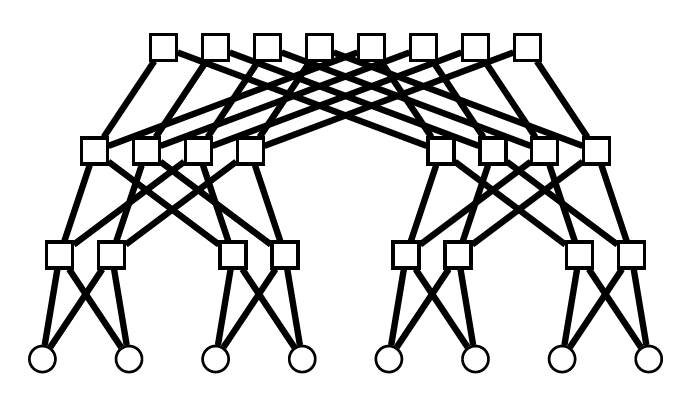
\includegraphics[width=10cm]{benes_network.png}
\caption[A folded Bene\v{s} network connecting eight processors]{A folded Bene\v{s} network connecting eight processors. \cite{Han14}}
\label{fig:benes}
\end{figure}

Figure \ref{fig:benes} shows an example of the layout of nodes and edges in a folded Bene\v{s} network. The eight circular nodes at the bottom of the network represent eight processors which use the network for communication. Coming out from each of the processors are two interconnects which link the processors to the first layer of intermediate nodes in the network. These links -- and all of the others in the network -- are bidirectional which means that communication data can travel either towards the processors or away from them. Each of the intermediate square nodes in figure \ref{fig:benes} represents a $2 \times 2$ switch, the design of which is described in more detail in section \ref{sec:switch_design}. Where $p$ is the number of processors connected to the network, there are $\mathrm{log}\ p$ layers of $p$ switches culminating in a partially connected network, which means that -- using packet switching and credit-based control flow -- any processor in the network can communicate with any other processor in the network.

Bene\v{s} networks are rearrangeable and provide non-blocking communication between processors. In terms of universality, the number of intermediate switch nodes in the network means that the network could take the physical form of the other topologies discusses in section \ref{sec:topologies}, and emulate the behaviour of them. In terms of scalability, the number of switch layers included in the network is dependent on the number of connected processors. This means that, provided the number of switch layers is correctly updated, that an arbitrary number of processors can be connected to the network and it will still function correctly. In the situation where the number of processors is not a power of two, non-functioning placeholders can be used to bring the number of source nodes up to the next power of two without affecting the behaviour of the network. This means that Bene\v{s} networks are both universal and scalable, making them ideal for use in the emulation.

\subsection{Network switch design}
\label{sec:switch_design}

In a folded Bene\v{s} network, each switch is connected to two core-facing links (which are located closer to the processors), and two edge-facing links (which are located further away from the processors). This means that the switches are referred to as $2 \times 2$ switches, or crossbar switches. A diagram of how communication data can pass through these switches when being transmitted through the network is displayed below.

\begin{figure}[H]
\centering
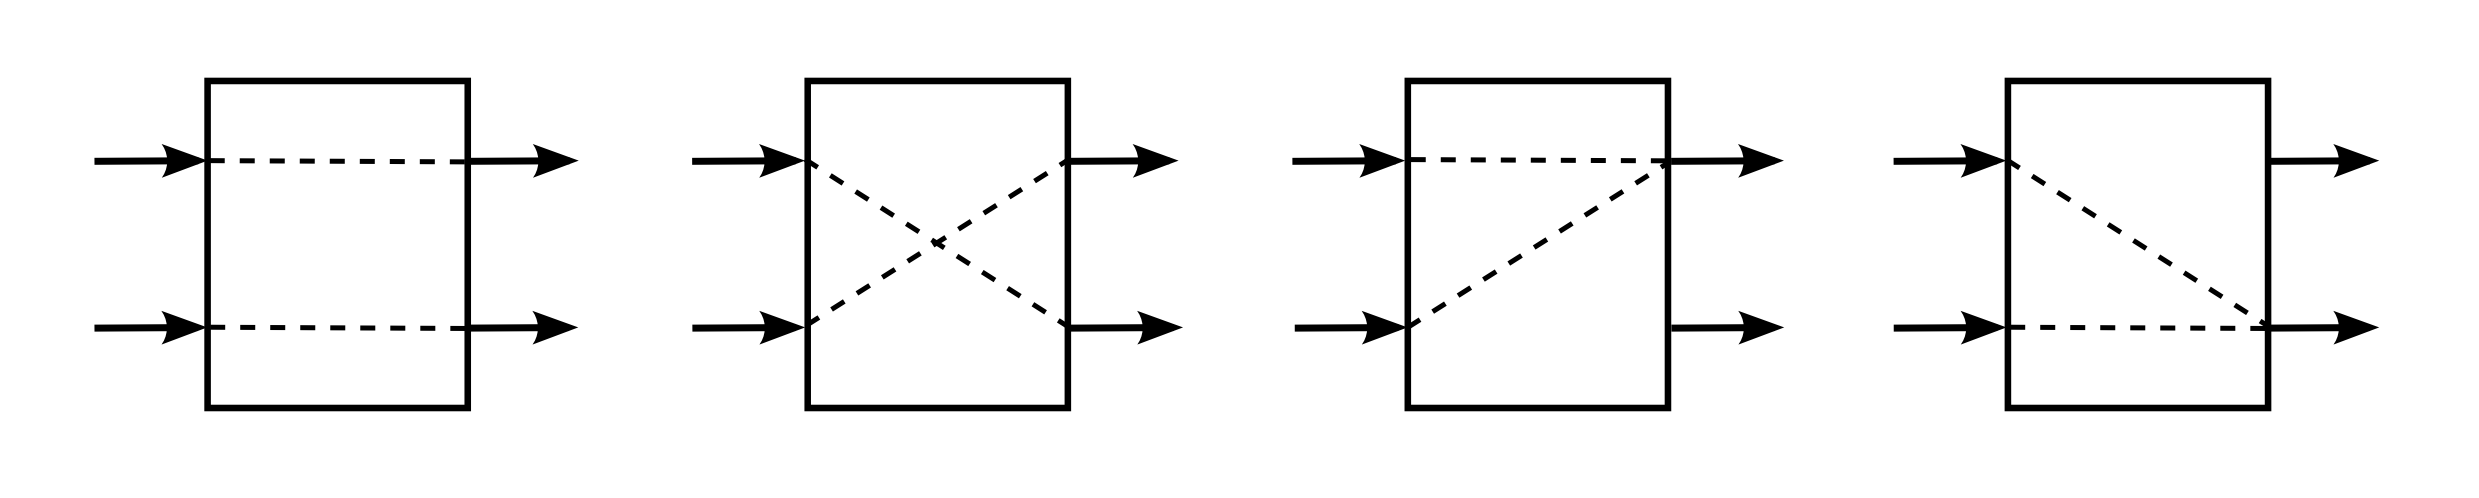
\includegraphics[width=\textwidth]{switch_directions.png}
\caption[The possible permutations of data flow through a one-way crossbar switch]{The possible permutations of data flow through a one-way crossbar switch.}
\label{fig:switch_direcitons}
\end{figure}

Figure \ref{fig:switch_direcitons} shows the four possible scenarios of how concurrent communication data can be handled by crossbar switches which use unidirectional input and output links. However, in the case of folded Bene\v{s} networks, bidirectional links are used which means that each switch has four input/output opportunities at a given time. This could equate to four packets being sent from the switch, four packets being received by the switch, or a mixture of the two.

In the case of the two rightmost permutations in figure \ref{fig:switch_direcitons}, the two input packets are shown to require the same output link to continue their transmission. This results in a collision in the network, as both packets cannot use the link at the same time. For this scenario, buffer space can be allocated to each output link of the switch so that communication data involved in the collision can be stored inside the switch until the link becomes free again and transmission of the stored communication data can continue. This means that data packets that collide do not have to be re-sent completely by their source processor, saving time and therefore increasing the efficiency of the network.

\begin{figure}[H]
\centering

\includegraphics[width=\textwidth]{switch_buffer.png}
\caption[A one-way crossbar switch with a 5-space buffer for each output link]{A one-way crossbar switch with a 5-space buffer for each output link.}
\label{fig:switch_buffer}
\end{figure}

Figure \ref{fig:switch_buffer} shows how buffer space can be used in a one-way crossbar switch. In the case of folded Bene\v{s} networks, there are four output links meaning there are four buffers included inside the switch.

\subsection{Routing algorithm design}
\label{sec:routing_design}

The choice of routing algorithm used to determine which paths the communication data takes through the network is essential for reducing the number of collisions that occur. After considering many possibilities, an algorithm was chosen that allows parallel routing of both full and partial permutations through the network where, for a single permutation at least, it is \textit{guaranteed} that no collisions will occur while the data is being transmitted. 

To describe how this algorithm carries out collision-free permutation routing, its application on a slightly modified Bene\v{s} network, shown in figure \ref{fig:benes_sectioned}, is discussed. The same principles of the algorithm can then be applied to the folded Bene\v{s} network described in section \ref{sec:network_design}.

\begin{figure}[H]
\centering
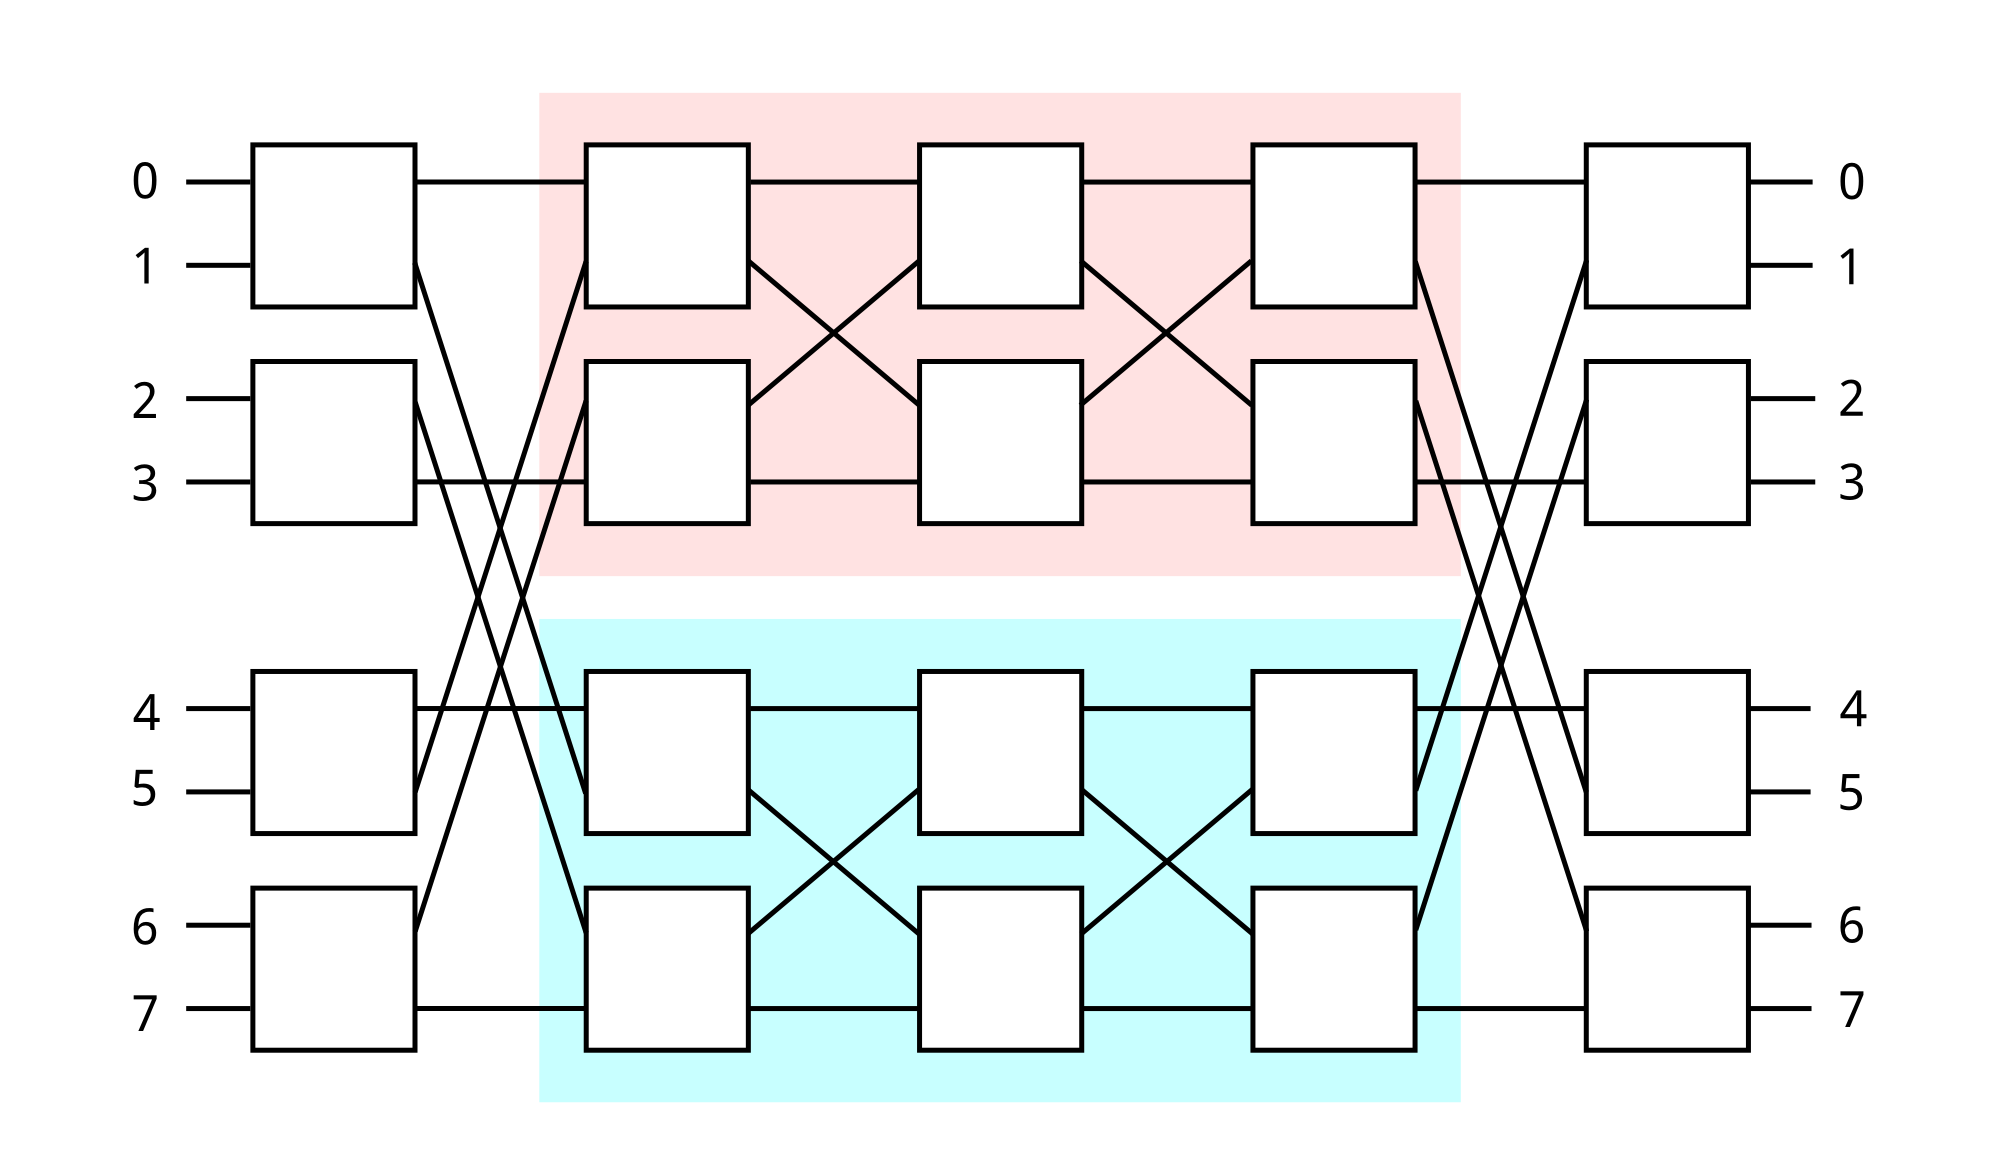
\includegraphics[width=\textwidth]{benes_sectioned.png}
\caption[A slightly modified Bene\v{s} network with two sections highlighted]{A slightly modified Bene\v{s} network with two sections highlighted.}
\label{fig:benes_sectioned}
\end{figure}

The Bene\v{s} network shown in figure \ref{fig:benes_sectioned} can be thought of as the unidirectional equivalent of the folded Bene\v{s} network described in section \ref{sec:network_design} but with a slightly different link ordering. The numbers on the left of the diagram represent the source processors that send communication data packets, and the numbers on the right of the diagram represent the destination processors that the communication data is being sent to. An important feature of Bene\v{s} networks is specifically highlighted by the pink and blue sections in figure \ref{fig:benes_sectioned}. It can be seen that once a packet of communication data has entered one of these sections, it remains in that section until the end of the section is reached. This feature is important for the routing algorithm described below. It is also noteworthy that each of the pink and blue sub-networks is in fact its own Bene\v{s} network -- a fact that can be extended to every layer of switches in the network -- meaning that the network is simply a recursion of itself.

The routing algorithm that can be used to carry out collision-free permutation routing on the network shown in figure \ref{fig:benes_sectioned} is described by the following:
\begin{enumerate}[leftmargin=*,labelindent=15pt,label=\bfseries \arabic*.]
	\item Take an empty, partial, or full permutation as input.
	\item Take the $i^{th}$ communication from the permutation and trace a front path from the source processor to the first switch it encounters in the network. If the switch has not previously handled any communication data for this permutation, set the packet route towards the first output link in the switch. If the switch has already handled a packet of communication data, set the packet route towards the second output link in the switch.
	\item For the same communication, trace a back path from the destination processor to the first switch it encounters on the network (in reality, the last switch that the packet will pass through during communication). Once inside the switch, set the route of the back path to mirror the direction that the front path was sent towards. This will result in both paths being directed into the same closed sub-network as shown by the highlighted sections in figure \ref{fig:benes_sectioned}.
	\item Repeat steps 2-3 for every communication in the permutation to calculate the first pairs of front and back path routes. Because each switch takes a maximum of two input packets, no collisions can occur as each packet is routed a towards a different output link by definition.
	\item Repeat steps 2-4, but this time continuing the front and back paths for each communication towards the centre of the network one layer of switches at a time.
	\item Once the front and back paths reach the same switch in the centre layer of the network, the route is complete.
\end{enumerate}

By following this iterative algorithm, routes through the network can be built up step by step until complete routes for the whole permutation are calculated. Not only does this ensure that each packet of communication data can be routed from the correct source processor to the correct destination processor, it also ensures that there are no collisions of communication data within the network. An example of the routes calculated from an arbitrary full permutation using this algorithm is shown below in figure \ref{fig:benes_full_perm}.

\begin{figure}[H]
\centering
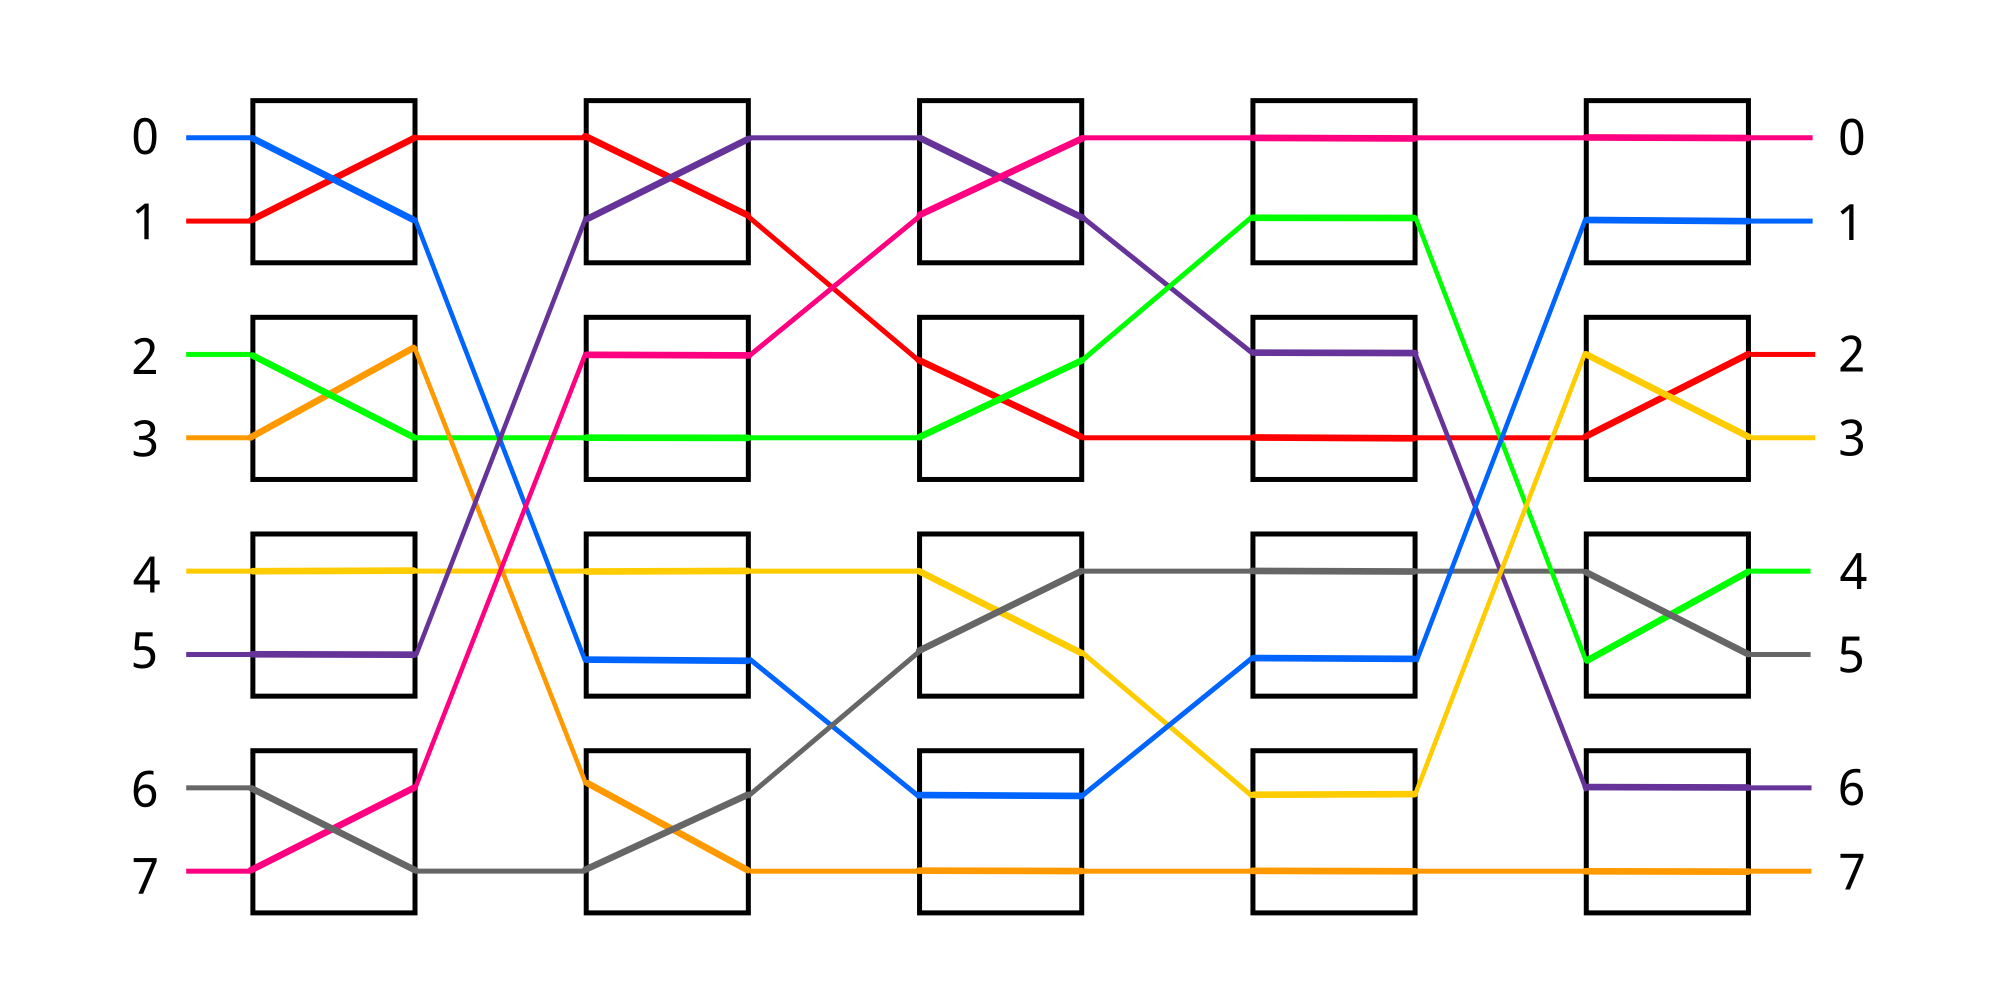
\includegraphics[width=\textwidth]{benes_full_perm.png}
\caption[Routing a full permutation]{Routing a full permutation.}
\label{fig:benes_full_perm}
\end{figure}

Until now, the workings of the algorithm have be described using a slightly modified Bene\v{s} network as a reference. This has been done for clarity. It is easier to demonstrate routing on unidirectional links in an unfolded Bene\v{s} network, but the same principles apply on a folded Bene\v{s} network with bidirectional links. In a single permutation, all of the packets of communication data are at the same switch layer at a time, meaning that no additional collisions can occur when the packets reach the outermost switch layer and the direction of transmission to changed to point towards the destination processors. Additionally, it is easier to demonstrate that the Bene\v{s} network is split into distinct sections after each layer of switches (as shown by the pink and blue highlighting in figure \ref{fig:benes_sectioned}) using a slightly modified link layout between switch layers in the network. This modified layout is essentially a mirror image of the layout to be used in the emulation, which means that these distinct sections after each layer of switches still exist, but they are not as easy to split into clear physical groupings as those shown in figure \ref{fig:benes_sectioned}. This difference in groupings has no affect on the algorithm.

All of this shows that the algorithm described above is able to calculate collision-free routes through a folded Bene\v{s} network, making it ideal for use in the emulation.

\subsection{Optimising the routing algorithm}
\label{sec:routing_optimisation}

The algorithm described in section \ref{sec:routing_design} is an optimal collision-free routing algorithm for the Bene\v{s} network described in figure \ref{fig:benes_sectioned}. However, the fact that a folded Bene\v{s} network will be used in the emulation means that some optimisation techniques can applied to the routing algorithm that take advantage of this difference in network structure to make communication more efficient without affecting the lack of collisions in the network.

The first optimisation that can be applied to the routing algorithm involves the spread of data packets across the two sub-networks that follow the first layer of switches. As the folded Bene\v{s} network contains two output links for each processor, each sent packet has an initial choice of which of the sub-networks to travel across. This means that if the packets are sent to alternating sub-networks, spread of traffic over the network is more likely to be uniform and the possibility of collisions between packets from different permutations is reduced.

A second optimisation that can be applied to the routing algorithm takes into account the bidirectional links in the folded Bene\v{s} network. The routing shown in figure \ref{fig:benes_full_perm} implies that every pair of front and back paths must reach the centre layer of switches before the route is complete. However, in a folded Bene\v{s} network, the front and back paths may encounter the same switch before reaching the final layer of switches. In this situation, there is no need for the pair of paths to be continued to the final layer of switches, so a shorter completed route can be allocated. This shorter path means that the communication data travels quicker through the network, making communication more efficient.

\subsection{Sourcing a suitable compiler}

It was mentioned in section \ref{sec:dependencies} that the functionality of the emulation is dependent on a compiler being sourced which can compile a parallel input program into instructions that are then distributed between the processors connected to the network and executed in parallel. During the network design phase, a solution to this problem was presented by David May, a Professor of Computer Science at the University of Bristol. David provided the source code of a compiler that is able to handle parallel code sections, and the source code of a serial processor that, with some modifications applied to it, could read and execute the instructions produced by the compiler. I am very grateful for David's contribution towards this thesis.

\subsection{Output of the compiler}

The compiler takes the source code of a parallel input program as input and produces binary file represented in hexadecimal as output, which is then available for the processors in the network to read and execute. In order to do this, the binary output file produced by the compiler must be understood so that the binary instructions it carries can be executed correctly by the processors in the network. An example of this binary output is given in figure \ref{fig:compiler_binary} below.


\begin{figure}[H]
\centering
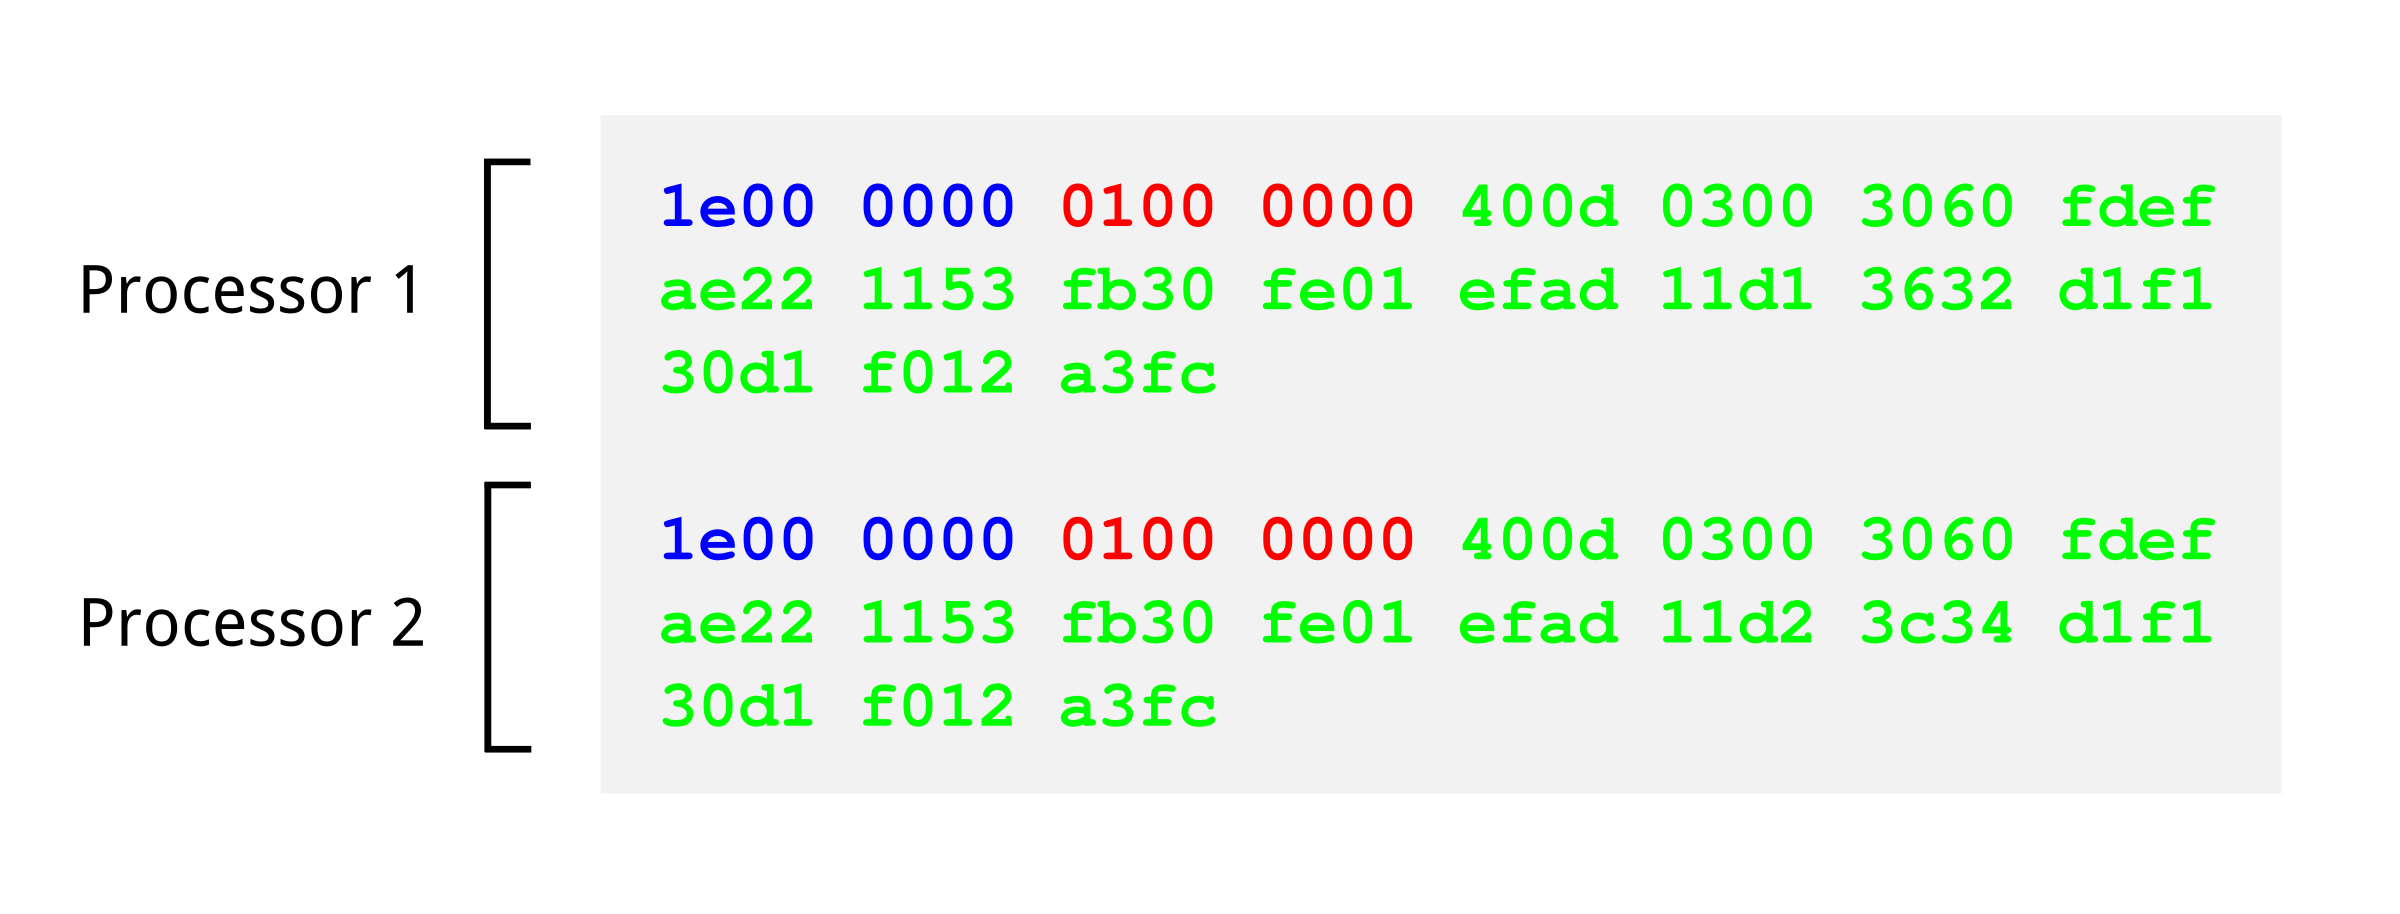
\includegraphics[width=15cm]{compiler_binary.png}
\caption[An example of binary output from the compiler]{An example of binary output from the compiler, with added sectioning and colouring.}
\label{fig:compiler_binary}
\end{figure}

It can be seen that the binary for each processor is split into three sections. The first section, represented by the blue font colour in figure \ref{fig:compiler_binary}, indicates the length of the binary string relevant to each processor, measured in bytes. This gives an indication of the positions in the binary that instructions for one processor stop and instructions for another processor start, meaning it is vital for the distribution of the different parts of the parallel program to their correct processors ready for parallel execution. The second section in the binary for each processor, represented by the red font colour, indicates the initial value of the program counter that the processor uses during execution of the program. The third section, represented by the green font colour, indicates the instructions that the processor carries out in order to execute the program correctly. Each instruction is made up of 8-bits: a 4-bit operation code and 4-bits of immediate data. Larger data can be handled using inter-register operations. 

This sequence of three binary sections is then repeated for every processor involved in the parallel input program, resulting in a full binary file ready to be executed by the emulation.

\subsection{Processor modifications}
\label{sec:processor_mods}

The processor that was provided with the compiler source code is designed to execute most of the instructions described in the binary output file that the compiler produces. A summary of the instruction set of this processor is included as \textbf{Appendix B}. However, the processor was designed as a serial processor which means that it has no communication capabilities, and that instructions for the sending of communication data to the network and the receiving of communication data from the network needed to be added. Additionally, the provided source code for the processor only accounted for a single instance of the processor, whereas the network requires multiple processors to function correctly. Provided that these features are added, the processor source code is suitable for integration with the network and can be included in the emulation. 

\newpage
\section{Implementation}

The following chapter describes how the emulation was created. The programming language chosen to code the emulation was C due to its speed, efficiency and the ease at which memory address manipulation can be carried out. The code also uses only the standard C libraries, making it portable across virtually all machines running Linux.

\subsection{Building the network}
\label{sec:imp_build_network}

The network is made up of two main building blocks: $2 \times 2$ crossbar switches and interconnects which link these switches together. These entities were created as individual data structures that interact with each other to facilitate traversal through the network.\\

\noindent\textbf{5.1.1 \ \ Link data structure}

\noindent The links are used to carry packets of communication data across the network. Each link can contain a maximum of one packet of data at a time, which is the reason that collisions of data packets in the network occur. This means that the Link data structure consists of a pointer to the data packet that it is currently transmitting, and if the link is vacant the pointer is set to null. For reasons regarding the emulated parallelism in the network, a second pointer to a temporary data packet is also included in the Link data structure. The function of this additional pointer is described in section \ref{sec:imp_parallelism}.\\

\noindent\textbf{5.1.2 \ \ Switch data structure}

\noindent The switches are used to direct the packets of communication data across the network towards their destination, following the route calculated for each packet by the routing algorithm. In a folded Bene\v{s} network, each switch connects four interconnects which can be used for both input and output of data packets to and from the switch. This means that the Switch data structure contains four instances of the Link data structure, which allow packets of communication data to move across the network. 

In the situation where two packets of communication data try to use the same link at the same time during transmission across the network, a collision occurs. This means that one of the data packets must wait for the link to become free again before it can continue its transmission. To facilitate the queuing of data packets for each output link in the switch, four buffer spaces are needed, which means that four instances of the Buffer data structure are also included as part of the Switch data structure.\\

\noindent\textbf{5.1.3 \ \ Buffer data structure}

\noindent The buffer for each of the output links in a switch is implemented as a cyclic buffer. This means that the Buffer data structure includes an array of data packets currently being stored in the buffer, a value indicating the index of the array that holds the next packet to be sent across the output link, a value indicating the index of the array where the next data packet to be input into the buffer should be placed, and a value that indicates the number of data packets currently being held in the buffer. The size of each buffer is variable, and is defined at the top of the code. The index values are variable, and change every time an input or output occurs. The count value can be used to indicate whether the buffer is empty or full; if the buffer is empty then it can simply be ignored, and if the buffer is full then it cannot accept any more data packets meaning that any additional data packets that require use of the output link that the buffer supplies must wait in the input link to the switch until space becomes available in the buffer. This functionality is referred to as credit-based flow control.\\

\noindent\textbf{5.1.4 \ \ Forming the network}

\noindent The main frame for the network is built up using these three data structures. The construction of this frame can be described in layers, where $n$ is the number of processors that the network will connect. Firstly, a bottom layer consisting of $2n$ links is initialised. These links will be used to connect the processors to the first layer of switches. Next, a layer consisting of $n$ switches is initialised and placed above the bottom layer of links. Each of the switches in this layer is then connected to two of the links in the layer below. Another layer consisting of a further $2n$ links is then initialised and placed above the first layer of switches, where each of the switches is connected to a further two links in the layer above. This layering process is continued until there are log($n$) layers of switches connected to log($n$) layers of links and a folded Bene\v{s} network as described in section \ref{sec:network_design} is formed.

\subsection{Creating the processors}

It was described in section \ref{sec:processor_mods} that an emulated processor was provided that can read and interpret the binary output of the provided compiler. A summary of the instruction set of this processor is included as \textbf{Appendix B}. However, to make this processor suitable for use in the emulation, some modifications to the processor were required. These modifications included adding input and output functionality which allows the processor to send and receive packets of communication data from the network, and adding the ability for multiple instances of the processor to be created so that more than one processor can be connected to the network.\\

\noindent\textbf{5.2.1 \ \ Adding the output instruction}

\noindent An output instruction is given by the compiler as the binary characters 0xF, which represents an operation, and 0x11 which represents an output operation. Directly before an output instruction, the processor takes the destination address of the packet of communication data to be sent, as well as the data itself, and stores this data in the processor's registers. When the following output instruction is read, the processor informs the routing algorithm that a calculated route for a packet of communication data is required, and it provides the routing algorithm with the details of the destination address and the data to be sent stored in the registers. Once this information has been passed on, the processor can immediately carry on executing its next instructions because the network is a non-blocking network. This means that computation can be carried out while packets are being sent across the network, which is part of a technique for increasing program efficiency called latency hiding.\\

\noindent\textbf{5.2.2 \ \ Adding the input instruction}

\noindent An input instruction is given by the compiler as the binary characters 0xF, which represents an operation, and 0x10 which represents an input operation. Directly before an input instruction, the processor takes the port number where the received packet will be placed, and the memory address of the variable that will be set as the data provided by the received packet.  When the following input instruction is read, the processor will check with the network adapter (described in section \ref{sec:imp_network_adapter}) whether a packet has been received at the specified port address. If the packet has been received, the processor takes the data provided by the packet and stores it in memory under the stated variable name, before continuing execution of its next instructions. If the packet has not been received at the specified port address, it is still being transmitted across the network. In this situation, the processor must wait until the packet is delivered before it can continue execution of its next instructions, which means that the input instruction is read over and over until the packet is delivered and the data it provides can be extracted and stored.\\

\noindent\textbf{5.2.3 \ \ Creating multiple processors}

\noindent Currently the processor works as a single entity. However, the network requires a variable number of processors to be connected to carry out parallel computation, which means that multiple instances of the processor are needed. To emulate this, arrays of the registers for each processor are initialised. An array of the memory blocks for each processor is also initialised, where each processor's individual set of instructions described in the binary file produced by the compiler are stored. This means that each processor has its own set of instructions stored in its own memory block, and can execute these instructions using its own registers, which indicates that the multiple processors are fully independent of one another and are suitable for connection to the network.

\subsection{Connecting the processors to the network}
\label{sec:imp_network_adapter}

Now that multiple emulated processors are available, they can be connected to the bottom layer of links described in section \ref{sec:imp_build_network} which joins them to the network. To do this, a data structure is needed that acts as a network adapter. This allows packets to be added to the network when a processor needs to send communication data, and packets to be removed from the network once the packet has been received by its destination processor.\\

\noindent\textbf{5.3.1 \ \ Network Adapter data structure}

\noindent The Network Adapter data structure consists of two Link data structures which connect the network adapter to the first layer of switches in the network, a port for next output packet to be added to the network, and an array of numbered ports where input packets can be stored until they are collected by the destination processor when an input instruction is read.

When an output instruction is read by a processor, the network adapter waits to receive a packet of communication data from the routing algorithm. Once this packet is received, it is added to the output port of the network adapter. The packet has now been introduced into the network, where it can travel along the path calculated by the routing algorithm towards its destination.

When a packet reaches its destination processor, it is removed from the network and stored in the specified port number in the network adapter. It remains stored in the port until an input instruction is read by the destination processor that requires the data inside the packet stored in that port. When this occurs, the data is removed from the port and used in the program currently being executed. If an input instruction is read by a processor which refers to an empty input port, the processor must wait until the required data arrives.

\subsection{Integrating the routing algorithm}

The routing algorithm is triggered when one of the processors reads an output instruction, which indicates that a calculated route though the network is required for a packet of communication data. Before calculating the route, the routing algorithm scans all of the other processors in the network for any other parallel output communications that are required. Using the source and destination addresses for all of the gathered communications, a permutation is formed which is then used by an implementation of the algorithm described in sections \ref{sec:routing_design} and \ref{sec:routing_optimisation} to calculate collision-free routes through the network for each communication in the permutation. 

Each calculated route is represented as three values: a count value, which indicates how many layers of switches the route traverses on its outward path before it changes direction and begins its inward path back towards the processors, a routing bit-string which indicates which of the output links connected to each switch encountered on the outward route are taken, and an addressing bit-string which indicates which of the output links connected to each switch encountered on the inward route are taken. For both bit-strings, a 0 represents a route though the leftmost output link, and a 1 represents a route though the rightmost output link. The least significant bit of both bit-strings represents the route taken at the first layer of switches, and the most significant bit represents the route taken at the last layer of switches before the direction of the route is reversed.\\

\noindent\textbf{5.4.1 \ \ Packet data structure}

\noindent Reference to the calculated route is required throughout each packet's traversal across the network, which means a Packet data structure is required. The Packet data structure consists of the count value and routing and addressing bit-strings created by the routing algorithm, as well as the source processor address, the destination processor address, the destination port number, the data being transmitted, and an indication of which direction the packet is currently travelling in. 

For every output instruction read by the processors, a new packet is created. Once all of the values in the Packet data structure have been set by the routing algorithm, the packet is passed to the network adapter where it is added to the network ready for transmission.

\subsection{Emulating the parallelism}
\label{sec:imp_parallelism}

The emulated hardware building blocks of the network are now fully connected, and can interact with each other. The final stage of the network implementation concerns the functionality of these hardware components when they are working together in parallel. The standard C libraries do not support parallel computation, so the parallelism is emulated using a timestep implementation where a single unit of time's worth of functionality is carried out by each component in the network in serial, before the next timestep is started and the process is repeated. This continues until all of the processors have executed their section of instructions given by the parallel input program. The total number of timesteps that are required to fully execute an input program gives an indication of the run time of the program.


description of processor timestep
routing algorithm in constant time
description of network timestep

\newpage
\section{Testing}



\newpage
\section{Results}



\newpage
\section{Conclusion}



\newpage
\section{References}

\begin{thebibliography}{30}

\bibitem[Adv08]{Adv08} Adve, S. V. et al. (November 2008). \textit{'Parallel Computing Research at Illinois: The UPCRC Agenda'}. Parallel@Illinois, University of Illinois at Urbana-Champaign.

\bibitem[Ben65]{Ben65} Bene\v{s}, V. E. (1965). \textit{Mathematical Theory of Connecting Networks and Telephone Traffic}. Mathematics in Science and Engineering. Academic Press.

\bibitem[Clo53]{Clo53} Clos, C. (March 1953). \textit{'A study of non-blocking switching networks'}. Bell System Technical Journal 32 (2): 406-424. doi:10.1002/j.1538-7305.1953.tb01433.x.

\bibitem[Dal87]{Dal87} Dally, W. J., Seitz, C. L. (May 1987). \textit{Deadlock-free message routing in multiprocessor interconnection networks}. Computers, IEEE Transactions on, 100 (5): 547-553.

\bibitem[Dal92]{Dal92} Dally, W. J. (March 1992). \textit{Virtual-channel flow control}. IEEE Transactions on Parallel and Distributed Systems, 3 (2): 194-205.

\bibitem[Dal03]{Dal03} Dally, W. J., Towles, B. (2003). \textit{Principles and Practices of Interconnection Networks}. Morgan Kaufmann.

\bibitem[Fly72]{Fly72} Flynn, M. J. (September 1972). \textit{'Some Computer Organizations and Their Effectiveness'}. IEEE Trans. Comput. C-21 (9): 948-960. doi:10.1109/TC.1972.5009071.

\bibitem[Got89]{Got89} Gottlieb, A. Almasi, G. (1989). \textit{Highly parallel computing}. Redwood City, Calif.: Benjamin/Cummings. ISBN 0-8053-0177-1.

\bibitem[Han14]{Han14} Hanlon, J. W. (March 2014). \textit{Scalable abstractions for general-purpose parallel computation}. p. 44-48, 62.

\bibitem[Hen11]{Hen11} Hennessy, J. L., Patterson, D. A. (2011). \textit{Computer Architecture: A Quantitative Approach}. Online appendix F, retrieved from http://booksite.elsevier.com/9780123838728/references.php

\bibitem[Iba08]{Iba08} Ibaroudene, Djaffer. (Spring 2008). \textit{'Parallel Processing, EG6370G: Chapter 1, Motivation and History'}. St. Mary's University, San Antonio, TX.

\bibitem[Jon97]{Jon97} Jones, A. M. et al. (1997). \textit{The Network Designer's Handbook}. IOS Press, 1st edition.

\bibitem[Lam04]{Lam04} Lammle, T. (2004). \textit{CCNA Study Guide} (Fourth edition). Sybex Inc. ISBN 0-7821-4311-3.

\bibitem[Moo65]{Moo65} Moore, G. E. (1965). \textit{'Cramming more components onto integrated circuits'}. Electronics Magazine. p. 4.

\bibitem[Sut05]{Sut05} Sutter, H. (March 2005). \textit{'The free lunch is over'}. Dr Dobb's Journal, 30(3). Online version, updated August 2009.

\bibitem[Toy86]{Toy86} Toy, W., Zee, B. (1986). \textit{Computer Hardware/Software Architecture}. Prentice Hall. ISBN 0-13-163502-6.

\bibitem[Val90]{Val90} Valiant, L. G. (1990). \textit{General purpose parallel architectures}. In Handbook of theoretical computer science (vol. A): algorithms and complexity, p. 943-973. MIT Press.

\end{thebibliography}

\newpage
\section*{Appendix A: User Manual}
\addcontentsline{toc}{section}{Appendix A: User Manual}


\newpage
\section*{Appendix B: Summary of Processor Instruction Set}
\addcontentsline{toc}{section}{Appendix B: Summary of Processor Instruction Set}

This appendix describes a summary of the instruction set associated with the unmodified serial processor. The modifications carried out to to the processor to add parallelism to its capabilities are described in sections 4 and 5. This document was written by David May.

\subsection*{Background}
\setlength{\parindent}{0in}

The architecture described here is specifically designed as a very
simple component processor for multiprocessors. In area, it 
would occupy less area on silicon than $16kbytes$ of memory,
allowing a manufacturable chip to contain thousands 
of  processors.
Further, its instruction set requires a very small compiler to
generate near-optimal code, so it is practical to compile 
on-the-fly as programs are input. This may be important 
as it makes it practical to broadcast programs to 
thousands of processors, each of which compiles the
incoming program in the context of its local state. The main
features of the instruction set are: 

\begin{itemize}

\item Short instructions are provided to allow efficient
access to the stack and other data regions allocated
by compilers; these also provide efficient branching and 
subroutine calling. The short instructions have been chosen on 
the basis of extensive evaluation to meet the needs of 
modern compilers. 

\item The memory is word addressed; however the 
instructions are all single byte so instruction 
addresses refer to a specific byte position within a 
word. 

\item The same instruction set can be used for processors 
with different wordlengths; the only requirement is that 
the wordlength is a number of bytes. 

\item The processor has a small number of registers. 
Some registers are used for specific purposes such as 
accessing the stack or building large constants. 

\item Instructions are easy to decode. 

\end{itemize}

All instructions are 8-bit; each instruction contains 4 bits representing
an operation and 4 bits of immediate data. A special instruction, OPR
causes its operand to be interpreted as an inter-register operation. 
Instruction prefixes are used to extend the range of immediate operands 
and to provide more inter-register operations. 

The prefixes are:

\begin{itemize}
\item PFIX which concatenates its 4-bit immediate with the 4-bit immediate
of the next 8-bit instruction.
\item NFIX which complements its its 4-bit immediate and then concatenates 
the result with the 4-bit immediate of the next 8-bit instruction. 
\end{itemize}

The prefixes are inserted automatically by compilers
and assemblers. 

The normal state of a processor is represented by 5 registers.
Two of the registers are operated as a stack and used to hold the
sources and destination of inter-register operations. 

\begin{tabular}{ll}
{\bf register} & {\bf use}\\
&\\
$pc$ & the program counter\\
&\\
$sp$ & the stack pointer\\
$oreg$ & the operand register\\
&\\
$areg$ & the first register in the operand stack \\
$breg$ & the second register in the operand stack
\end{tabular}

\subsection*{Instruction Issue and Execution}

The processor core is intended to be implementable without
a pipeline to maximise responsiveness; this potentially allows
a very simple design. 

Note that the instructions are all 8-bit, so that on a 
32-bit implementation four instructions are fetched every cycle.
As typically less than 40\% of instructions require a memory
access, it is therefore practical to support the processor
using a simple unified memory system.

Each processor has a short instruction buffer which is one 
word long. The rules for performing an instruction 
fetch are as follows:

\begin{itemize}
\item Any instruction which requires data-access performs
it during the memory access stage.
\item Branch instructions fetch their branch target instructions
during the memory access stage. 
\item Any other instruction (such as ALU operations) 
performs an instruction fetch if it is the
last instruction in the instruction buffer. 
 \item If the instruction buffer is empty when an instruction 
should be issued, a special {\it no-op} is issued; this 
will load the instruction buffer. 
\end{itemize}

\subsection*{Instruction set Notation and Definitions}

In the following description

\begin{tabular}{ll}
$Bpw$ &is the number of bytes in a word \\
$bpw$ & is the number of bits in a word \\
&\\
$mem$ & represents the memory \\
&\\
$pc$ & represents the program counter\\
$sp$ & represents the stack pointer\\
$oreg$ & represents the operand register\\
$areg$ & represents the first stack register\\
$breg$ & represents the second stack register\\
&\\
$u4$ & is a 4-bit unsigned source operand in the range $[0:15]$\\
\end{tabular}

\subsection*{Data access}

The data access instructions fall into several groups. One of these
provides access via the stack pointer.

\begin{tabular}{lll}
LDWSP & $areg, breg \leftarrow mem[sp + oreg], areg$& load word from stack \\ 
STWSP & $mem[sp + oreg], areg \leftarrow areg, breg $& store word to stack  \\
LDAWSP & $areg, breg \leftarrow sp + oreg, areg $& load address of word in stack  
\end{tabular}

Access to constants and program addresses is provided by instructions which 
either load values directly or enable them to be loaded from a location in 
the program: 

\begin{tabular}{lll}
LDC  & $areg, breg \leftarrow oreg, areg $& load constant  \\
LDAP & $areg, breg \leftarrow pc + oreg, areg $& load address in program  
\end{tabular}

Access to data structures is provided by instructions which combine an
address with an offset:

\begin{tabular}{lll}
LDWI  & $areg \leftarrow mem[areg + oreg]$& load word  \\
STWI  & $mem[areg + oreg] \leftarrow breg$& store word   
\end{tabular}


\subsection*{Expression evaluation}

\begin{tabular}{lll}
ADDC & $ areg \leftarrow areg + oreg $ & add constant\\  
ADD & $ areg \leftarrow breg + areg $ & add \\  
SUB & $ areg  \leftarrow breg - areg $ & subtract \\  
&&\\
EQC & $ areg \leftarrow areg = oreg $ & equal constant \\  
EQ & $ areg \leftarrow breg = areg  $ & equal \\  
LSS & $ areg  \leftarrow breg  <_{sgn} areg $ & less than signed \\  
&&\\
AND & $ areg \leftarrow breg \wedge areg $ & and \\  
OR  & $ areg \leftarrow breg  \vee areg $ & or \\  
XOR & $ areg \leftarrow breg \oplus areg $& exclusive or \\
NOT & $ areg  \leftarrow -1 \oplus areg $& not\\
&&\\
SHL & $ areg \leftarrow breg \ll areg $ & logical shift left \\  
SHR & $ areg \leftarrow breg \gg areg $ & logical shift right  \\  
\end{tabular}


\subsection*{Branching, jumping and calling}

The branch instructions include conditional and unconditional relative 
branches. A branch using an offset in the stack is provided to 
support jump tables.

\begin{tabular}{lll}
BR   & $ pc \leftarrow pc + oreg $& branch relative unconditional \\
BRT & $\mathrm{if}\; areg \;\mathrm{then}\; pc \leftarrow pc + oreg $ &branch relative true\\
&&\\
BRX & $pc, areg \leftarrow areg, breg$ &branch absolute\\
\end{tabular}

The procedure calling instruction uses a program address in the stack
to determine a subroutine entry point, leaving the return address on the 
stack. The RET instruction can also be used simply to branch to 
a program address on the stack.

\begin{tabular}{lll}
CALL & $mem[sp], pc, areg \leftarrow pc, areg, breg $ &call subroutine\\
RET   & $pc \leftarrow mem[sp] $ & return from subroutine
\end{tabular}

Typically, the stack is initialised to a high address in memory and is
extended on subroutine entry and contracted on exit. 
The instructions to support this are shown below.

\begin{tabular}{lll}
SETSP & $sp, areg  \leftarrow areg, breg $& set stack pointer \\
ADJ & $sp \leftarrow sp + oreg $& adjust stack
\end{tabular}


\newpage
\subsection*{Instruction summary}

\begin{tabular}{lll}
LDWSP & $areg, breg \leftarrow mem[sp + oreg], areg$& load word from stack \\ 
STWSP & $mem[sp + oreg], areg \leftarrow areg, breg $& store word to stack  \\
LDAWSP & $areg, breg \leftarrow sp + oreg, areg $& load address of word in stack  \\
LDC  & $areg, breg \leftarrow oreg, areg $& load constant  \\
LDAP & $areg, breg \leftarrow pc + oreg, areg $& load address in program  \\
LDWI  & $areg \leftarrow mem[areg + oreg]$& load word  \\
STWI  & $mem[areg + oreg] \leftarrow breg$& store word   \\
ADDC & $ areg \leftarrow areg + oreg $ & add constant\\  
EQC & $ areg \leftarrow areg = oreg $ & equal constant \\  
BR   & $ pc \leftarrow pc + oreg $ & branch relative unconditional \\
BRT& $\mathrm{if}\; areg \;\mathrm{then}\; pc \leftarrow pc + oreg $ &branch relative true\\
ADJ & $sp \leftarrow sp - oreg $& adjust stack\\
&&\\
ADD & $ areg \leftarrow breg + areg $ & add \\  
SUB & $ areg  \leftarrow breg - areg $ & subtract \\  
EQ & $ areg \leftarrow breg = areg  $ & equal \\  
LSS & $ areg  \leftarrow breg  <_{sgn} areg $ & less than signed \\  
AND & $ areg \leftarrow breg \wedge areg $ & and \\  
OR  & $ areg \leftarrow breg  \vee areg $ & or \\  
XOR & $ areg \leftarrow breg \oplus areg $& exclusive or \\
NOT & $ areg  \leftarrow -1 \oplus areg $& not\\
SHL & $ areg \leftarrow breg \ll areg $ & logical shift left \\  
SHR & $ areg \leftarrow breg \gg areg $ & logical shift right  \\  
BRX & $pc, areg \leftarrow areg, breg$ &branch absolute\\
CALL & $mem[sp], pc, areg \leftarrow pc, areg, breg $ &call subroutine\\
RET   &  $pc \leftarrow mem[sp] $ & return from subroutine\\
SETSP & $sp, areg  \leftarrow areg, breg $& set stack pointer \\
&&\\             
BOOT  &$ load()$& boot processor \\
                &$ pc, sp \leftarrow mem[0], memhigh$ \\
\end{tabular}


\end{document}